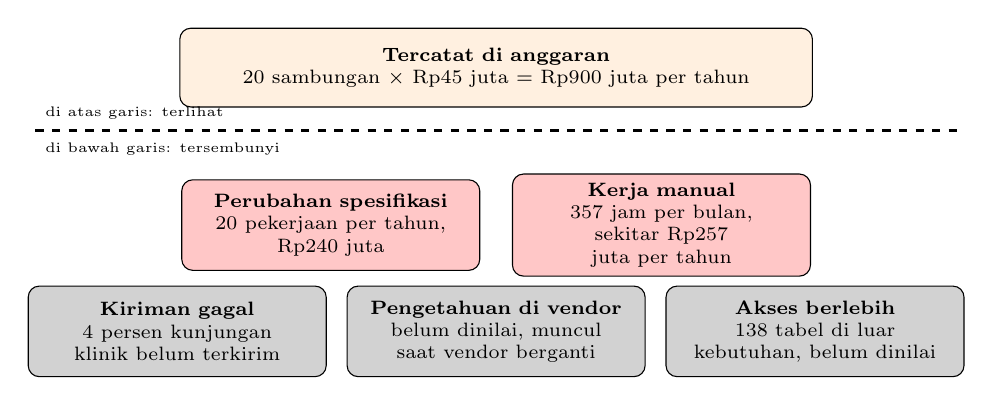
\begin{tikzpicture}[
  font=\scriptsize,
  terlihat/.style={draw, rounded corners, fill=orange!12, text width=7.8cm,
                   minimum height=1.0cm, align=center},
  dihitung/.style={draw, rounded corners, fill=red!22, text width=3.55cm,
                   minimum height=1.15cm, align=center},
  belum/.style={draw, rounded corners, fill=gray!35, text width=3.55cm,
                minimum height=1.15cm, align=center},
  ket/.style={font=\tiny, align=left, anchor=west}
]
  % Garis air memisahkan biaya yang tercatat dari biaya yang tidak terlihat di anggaran.
  \node[terlihat] at (5.85,1.0)
    {\textbf{Tercatat di anggaran}\\20 sambungan $\times$ Rp45 juta = Rp900 juta per tahun};
  \draw[dashed, thick] (0,0.2) -- (11.7,0.2);
  \node[ket] at (0,0.42) {di atas garis: terlihat};
  \node[ket] at (0,-0.04) {di bawah garis: tersembunyi};

  \node[dihitung] at (3.75,-1.0)
    {\textbf{Perubahan spesifikasi}\\20 pekerjaan per tahun,\\Rp240 juta};
  \node[dihitung] at (7.95,-1.0)
    {\textbf{Kerja manual}\\357 jam per bulan,\\sekitar Rp257 juta per tahun};

  \node[belum] at (1.8,-2.35)
    {\textbf{Kiriman gagal}\\4 persen kunjungan klinik belum terkirim};
  \node[belum] at (5.85,-2.35)
    {\textbf{Pengetahuan di vendor}\\belum dinilai, muncul saat vendor berganti};
  \node[belum] at (9.9,-2.35)
    {\textbf{Akses berlebih}\\138 tabel di luar\\kebutuhan, belum dinilai};
\end{tikzpicture}
